\section*{The number of solutions}

\begin{myConceptSteps}{
    To find how many solutions a system has\dots
}
    \myStep{Intersections}{
        Look at the points of \gap{intersection}.
    }
    \myStep{count}{
        \gap{Count} how many there are. (If you can!)
    }
    \myStep{possibilities}{\LARGE
        \begin{itemize}
            \item {\bfseries\itshape no solutions}:
                \vskip1em
                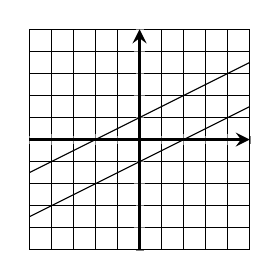
\begin{tikzpicture}
                    \begin{axis}[
                        width=2in,
                        grid=both,
                        grid style={solid,black},
                        axis x line = middle,axis y line = middle,
                        axis line style = {very thick},
                        axis equal image,
                        % xtick distance = 2, ytick distance = 2,
                        xmin = -5, xmax = 5,
                        ymin = -5, ymax = 5,
                        minor tick num = 1,
                        yticklabels={,,},
                        xticklabels={,,},
                        ]
                        \addplot[
                            no marks,
                            % only marks,
                            % mark=*,
                            % mark size = 0.1cm,
                            ] { 0.5*x -1 };
                            \addplot[
                                no marks,
                                % only marks,
                                % mark=*,
                                % mark size = 0.1cm,
                                ] { 0.5*x + 1 };
                        \end{axis}
                \end{tikzpicture}
            \item {\bfseries\itshape infinitely many solutions}:
            \vskip1em
            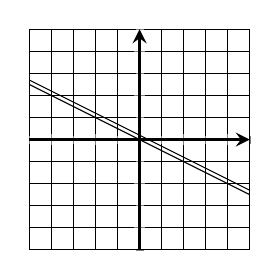
\begin{tikzpicture}
                \begin{axis}[
                    width=2in,
                    grid=both,
                    grid style={solid,black},
                    axis x line = middle,axis y line = middle,
                    axis line style = {very thick},
                    axis equal image,
                    % xtick distance = 2, ytick distance = 2,
                    xmin = -5, xmax = 5,
                    ymin = -5, ymax = 5,
                    minor tick num = 1,
                    yticklabels={,,},
                    xticklabels={,,},
                    ]
                    \addplot[
                        no marks,
                        % only marks,
                        % mark=*,
                        % mark size = 0.1cm,
                        ] { -0.5*x };
                    \addplot[
                        no marks,
                        % only marks,
                        % mark=*,
                        % mark size = 0.1cm,
                        ] { -0.5*x + 0.2 };
                    \end{axis}
            \end{tikzpicture}
        \item only a {\bfseries\itshape few solutions}:
        \vskip1em
        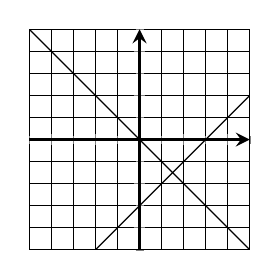
\begin{tikzpicture}
            \begin{axis}[
                width=2in,
                grid=both,
                grid style={solid,black},
                axis x line = middle,axis y line = middle,
                axis line style = {very thick},
                axis equal image,
                % xtick distance = 2, ytick distance = 2,
                xmin = -5, xmax = 5,
                ymin = -5, ymax = 5,
                minor tick num = 1,
                yticklabels={,,},
                xticklabels={,,},
                ]
                \addplot[
                    no marks,
                    % only marks,
                    % mark=*,
                    % mark size = 0.1cm,
                    ] { x-3 };
                \addplot[
                    no marks,
                    % only marks,
                    % mark=*,
                    % mark size = 0.1cm,
                    ] { -x };
                \end{axis}
        \end{tikzpicture}
        \hspace{0.5in}
        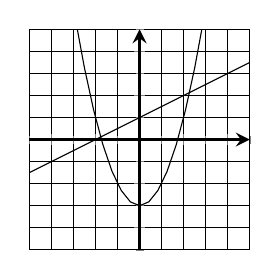
\begin{tikzpicture}
            \begin{axis}[
                width=2in,
                grid=both,
                grid style={solid,black},
                axis x line = middle,axis y line = middle,
                axis line style = {very thick},
                axis equal image,
                % xtick distance = 2, ytick distance = 2,
                xmin = -5, xmax = 5,
                ymin = -5, ymax = 5,
                minor tick num = 1,
                yticklabels={,,},
                xticklabels={,,},
                ]
                \addplot[
                    no marks,
                    % only marks,
                    % mark=*,
                    % mark size = 0.1cm,
                    ] { x^2 -3 };
                \addplot[
                    no marks,
                    % only marks,
                    % mark=*,
                    % mark size = 0.1cm,
                    ] { 0.5*x+1 };
                \end{axis}
        \end{tikzpicture}
\end{itemize}
    }
\end{myConceptSteps}
